\documentclass{article}
\usepackage{../../tpack/document/tpack}


\title{MI201 - Apprentissage Automatique}
\project{Résumé Théorique - SVM}
\author{Guilherme Nunes Trofino}
\authorRA{2022-2024}


\makeatletter
\begin{document}\selectlanguage{french}
\maketitle
\setlength{\parindent}{0pt}

\newpage\tableofcontents

\section{Introduction}
\subfile{../../intro.tex}

\section{Apprentissage}
\subsection{Algorithme}
On considère que l'algorithme peut être définie par la définition suivante:
\begin{definition}
    Algorithme discriminative qui vise divise les données pour un hyperplan avec deux approches possibles:
    \begin{enumerate}[rightmargin = \leftmargin]
        \item \textbf{Merge Souple}:
        \begin{definition}
            gets right, very right
        \end{definition}
        On peut noter les caractéristiques suivants:
        \begin{itemize}[noitemsep]
            \item \textbf{petit} C;
            \item \textbf{large} marge;
        \end{itemize}

        \item \textbf{Merge Rigide}:
        \begin{definition}
            getting everything right
        \end{definition}
        On peut noter les caractéristiques suivants:
        \begin{itemize}[noitemsep]
            \item \textbf{grand} C;
            \item \textbf{petit} marge;
        \end{itemize}
    \end{enumerate}
    On peut comparer les approches avec le figure suivant:
    \begin{center}
        \begin{minipage}[t]{0.495\textwidth}
            \begin{figure}[H]
                \centering
                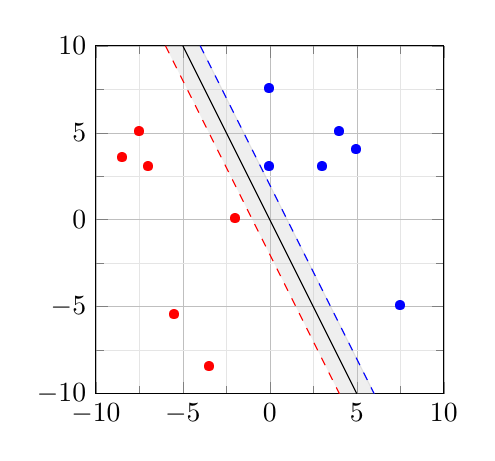
\begin{tikzpicture}
                    \begin{axis}[
                        xmin = -10, xmax = 10, % Axis Coordenates
                        ymin = -10, ymax = 10, % Axis Coordenates
                        % xlabel = {$x$}, % Axis Labels
                        % ylabel = {$y$}, % Axis Labels
                        % xtick = {, },      % Axis Ticks Potions
                        % ytick = {, },  % Axis Ticks Potions
                        % xticklabels = {, }, % Axis Ticks Labels
                        % yticklabels = {, }, % Axis Ticks Labels
                        % x label style = {at={(axis cs:{, })}, anchor=west},
                        % y label style = {at={(axis cs:{, })}, anchor=south, rotate=-90},
                        width  = 6cm,
                        height = 6cm,
                        grid = both,
                        grid style       = {line width=.1pt, draw=gray!20},
                        major grid style = {line width=.2pt, draw=gray!50},
                        minor tick num=1,
                        % axis lines = left, % Axis Position
                    ]
                    \node [red] at (-2.0, +0.0) {\textbullet};
                    \node [red] at (-7.5, +5.0) {\textbullet};
                    \node [red] at (-7.0, +3.0) {\textbullet};
                    \node [red] at (-8.5, +3.5) {\textbullet};
                    \node [red] at (-5.5, -5.5) {\textbullet};
                    \node [red] at (-3.5, -8.5) {\textbullet};
                    % \node [red] at (+2.0, +6.0) {\textbullet};
        
                    \node [blue] at (+0.0, +3.0) {\textbullet};
                    \node [blue] at (+0.0, +7.5) {\textbullet};
                    \node [blue] at (+3.0, +3.0) {\textbullet};
                    \node [blue] at (+5.0, +4.0) {\textbullet};
                    \node [blue] at (+4.0, +5.0) {\textbullet};
                    \node [blue] at (+7.5, -5.0) {\textbullet};
        
                    \draw[
                        color   =gray!75,
                        fill    =gray!50,
                        opacity =0.25
                    ] (-06, +10) -- (-04, +10) -- (+06, -10) -- (+04, -10);
                    \draw[blue,dashed] (axis cs:{-04, +10}) -- (axis cs:{+06, -10});
                    \draw[black]       (axis cs:{-05, +10}) -- (axis cs:{+05, -10});
                    \draw[red, dashed] (axis cs:{-06, +10}) -- (axis cs:{+04, -10});
                    \end{axis}
                \end{tikzpicture}
                \caption{SVM Merge Rigide}
            \end{figure}
        \end{minipage}
        \begin{minipage}[t]{0.495\textwidth}
            \begin{figure}[H]
                \centering
                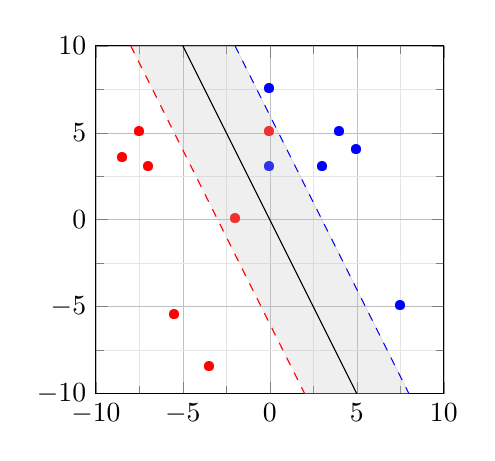
\begin{tikzpicture}
                    \begin{axis}[
                        xmin = -10, xmax = 10, % Axis Coordenates
                        ymin = -10, ymax = 10, % Axis Coordenates
                        % xlabel = {$x$}, % Axis Labels
                        % ylabel = {$y$}, % Axis Labels
                        % xtick = {, },      % Axis Ticks Potions
                        % ytick = {, },  % Axis Ticks Potions
                        % xticklabels = {, }, % Axis Ticks Labels
                        % yticklabels = {, }, % Axis Ticks Labels
                        % x label style = {at={(axis cs:{, })}, anchor=west},
                        % y label style = {at={(axis cs:{, })}, anchor=south, rotate=-90},
                        width  = 6cm,
                        height = 6cm,
                        grid = both,
                        grid style       = {line width=.1pt, draw=gray!20},
                        major grid style = {line width=.2pt, draw=gray!50},
                        minor tick num=1,
                        % axis lines = left, % Axis Position
                    ]
                    \node [red] at (-2.0, +0.0) {\textbullet};
                    \node [red] at (-7.5, +5.0) {\textbullet};
                    \node [red] at (-7.0, +3.0) {\textbullet};
                    \node [red] at (-8.5, +3.5) {\textbullet};
                    \node [red] at (-5.5, -5.5) {\textbullet};
                    \node [red] at (-3.5, -8.5) {\textbullet};
                    \node [red] at (+0.0, +5.0) {\textbullet};
        
                    \node [blue] at (+0.0, +3.0) {\textbullet};
                    \node [blue] at (+0.0, +7.5) {\textbullet};
                    \node [blue] at (+3.0, +3.0) {\textbullet};
                    \node [blue] at (+5.0, +4.0) {\textbullet};
                    \node [blue] at (+4.0, +5.0) {\textbullet};
                    \node [blue] at (+7.5, -5.0) {\textbullet};
        
                    \draw[
                        color   =gray!75,
                        fill    =gray!50,
                        opacity =0.25
                    ] (-8, +10) -- (-02, +10) -- (+8, -10) -- (+02, -10);
                    \draw[blue,dashed] (axis cs:{-02, +10}) -- (axis cs:{+8, -10});
                    \draw[black]       (axis cs:{-05, +10}) -- (axis cs:{+05, -10});
                    \draw[red, dashed] (axis cs:{-8, +10}) -- (axis cs:{+02, -10});
                    \end{axis}
                \end{tikzpicture}
                \caption{SVM Merge Souple}
            \end{figure}
        \end{minipage}
    \end{center}
    
    \begin{definition}
        \textbf{Hyperplan} est un plan en dimension plus grand. 
    \end{definition}
\end{definition}

Généralement on aura le comportement suivant:
\begin{table}[H]
    \centering\begin{tabular}{lll}
        C $\uparrow$   & biais $\downarrow$ & variance $\uparrow$\\
        C $\downarrow$ & biais $\uparrow  $ & variance $\downarrow$\\
    \end{tabular}
    \caption{Comportement SVM}
\end{table}

\subsubsection{Avantages}
Dans ce cas, cet algorithme 

\subsubsection{Incovenients}
Dans ce cas, cet algorithme 

\subsubsection{Applications}
Cet algorithme est souvent utilisé 


% \subsection{Initialization}
% \subsection{Visualization}
% \subsection{Training}



% \section{Prédiction}
% \subsection{Analyses}
\end{document}